\clearpage
%%
%% 2 x 3
%%
\begin{table}[htdp]
\caption[Fundamental projectors for matrix (a)]{Fundamental projectors for matrix (a) which has full rank. There are no \ns s. The range projectors are identity matrices and the \ns \ projectors are trivial.}
\begin{center}
\begin{tabular}{cc}
%
  $\Axey$ & $\Asyex$\\
%
  $\matrixa  \xthree = \ytwo$ &
  $\matrixat \ytwo   = \xthree$ \\[15pt]
%
$\Ap \ne \AinvL$ & $\paren{\A{*}}^{\sym} \ne \paren{\A{*}}^{-\mathrm{L}} $ \\
$\Ap \ne \AinvR$ & $\paren{\A{*}}^{\sym} \ne \paren{\A{*}}^{-\mathrm{R}} $ \\
%
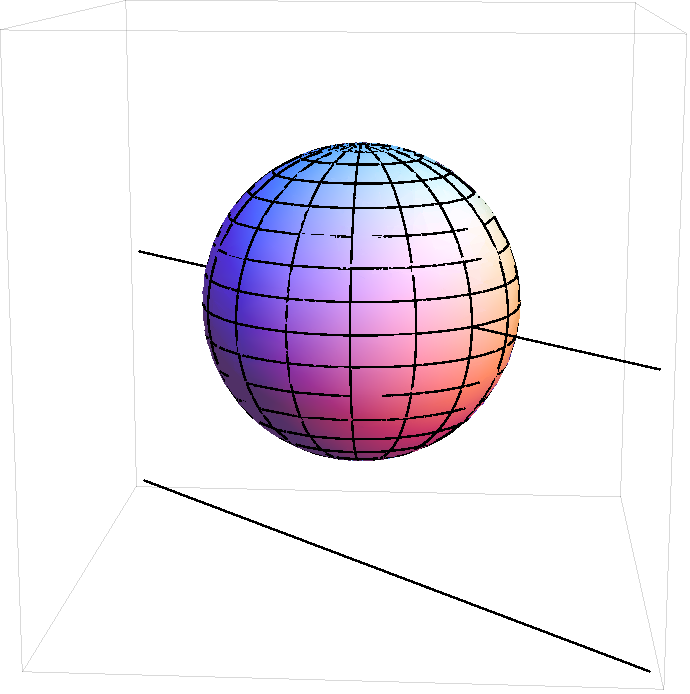
\includegraphics[ width = 2.in ]{images/projectors/a231} &
\includegraphics[ width = 2.in ]{images/projectors/"a231 s"} \\
%
 $\cmplx{3} \quad \mapsto \quad \cmplx{2}$ & 
 $\cmplx{2} \quad \mapsto \quad \cmplx{3}$\\[5pt]\hline
%%
\ \\
 $\pra  = \praa$  & $\pra  = \praas$ \\
\ \\
 $\pnas = \pnasa$ & $\pnas = \pnasas$ \\
\ \\
 $\pras = \prasa$ & $\pras = \prasas$ \\
\ \\
 $\pna  = \pnaa$  & $\pna  = \pnaas$
%
\end{tabular}
\end{center}
\label{tab:projector summary:a}
\end{table}

\endinput